%----------------------------------------------------------
\chapter{Программная реализация}\label{chap3_soft_architecture}
%----------------------------------------------------------
\section{Архитектура}\label{arch}

Редактор графов является web-приложением, соответственно весь программный код написан на языке JavaScript. Также стоит заметить, что приложение должно работать быстро, пользователь должен сразу видеть результат своих действий, будь то простое добавление очередной вершины или сохранение графа в формате aDOT, следовательно вся бизнес-логика должна выполняться на стороне клиента, то есть через JavaScript. В программном коде приложения для хранения графа реализован класс Graph, но в JavaScript концепция объектно-ориентированного программирование немного отличается от традиционной, поскольку в JavaScript ключевое слово class является лишь синтаксическим сахаром и на самом деле класс представляет из себя объект. Также стоит обратить внимание, что приватные методы класса остаются доступными внешнему коду, а сама приватность является лишь пометкой для разработчика, что этот метод не планируется вызывать через объект класса во внешнем коде.

В программном коде реализован один класс Graph, котырые предоставляет все необходимые методы для создания и работы в графом, UML -- диаграмма класса представлена на рисунке (\ref{fig:uml_chart}).

\begin{figure}[h!]
\center{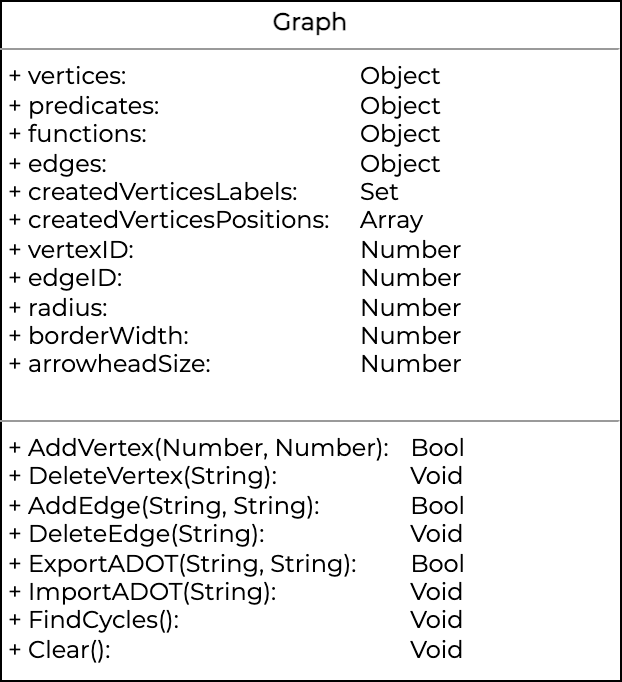
\includegraphics[width=0.5\linewidth]{images/UML.png}}
\caption{UML -- диаграмма класса Graph}
\label{fig:uml_chart}
\end{figure}

В UML -- диаграмме представлены только публичные методы класса Graph, которые вызываются из внешнего кода и реализуют всю бизнес-логику приложения. Для уменьшения объема диаграммы приватные методы были опущены.

\section{Реализация}

\subsection{Создание примитивов на странице}
Как было ранее сказано, редактор графов является web-приложением написанным на языке JavaScript. Для создания графа необходима возможность создавать простейшие примитивы: окружности, линии и прочее. JavaScript предоставляет несколько вариантов для решения этой задачи:
\begin{itemize}
	\item Использование HTML -- элемента canvas
	\item Работа с векторной графикой svg
\end{itemize}
Использование сanvas не подходит поскольку после создания примитива невозможно получить его свойства, а следовательно и отредактировать их. Таким образом, необходимо работать с векторной графикой svg, использование svg позволяет создавать примитивы, которые создаются как HTML теги с набором свойств, что позволяет редактировать или удалять созданные примитивы. Однако работать с svg без использования сторонних библиотек достаточно затруднительно, программный код сильно увеличивается и разработка функций для отрисовки примитивов занимает существенно больше времени. Для решения этой задачи подходит библиотека d3.js. Библиотека предоставляет набор инструментов для визуализации данных на странице, который состоит из нескольких дестяков небольших модулей, каждый из которых решает свою задачу. В программном коде возможности d3 используются для создания svg примитивов на странице, например создание вершины (листинг~\ref{lst:gm.exmpl.1}).

\begin{lstlisting}[label={lst:gm.exmpl.1}, caption={Пример создание вершины с использование библиотеки d3}, language=JavaScript]
  svg
    .append("circle")
    .attr("cx", x)
    .attr("cy", y)
    .attr("r", radius)
    .attr("stroke-width", borderWidth)
    .attr("id", id)
    .attr("fill", "#FFFFFF")
    .attr("stroke", "#000000")
    .attr("class", "vertex");
\end{lstlisting}

\subsection{Хранение информации о графовой модели}
Для того, чтобы иметь возможность гибко редактировать графовую модель, а также иметь возможность экспортировать граф в формат aDOT, необходимо хранить множество свойств графа. Так, при удалении вершины, помимо удаления примитивов со страницы, необходимо удалить всю информацию о вершине и связанных с ней ребрах, в противном случае при сохранении графа в формате aDOT в файле будет содержаться информация об уже удаленных вершинах или ребрах.

В разделе \ref{arch} описано, что вся бизнес-логика выполняеться на стороне клиента. Это касается и хранения данных. Все свойства графа хранятся в оперативной памяти. Для хранения большей части свойств в программном коде используются объекты. Объект - это мощная структура данных в javascript - используется для хранения коллекций разных значений. Рассмотрим на примере как храниться информаци о вершинах. В рассматриваемом примере (листинг~\ref{lst:gm.exmpl.2}) представлены хранимые в объекте свойства одной вершины из которой выходит одно ребро.

\begin{lstlisting}[label={lst:gm.exmpl.2}, caption={Пример хранение вершины в оперативной памяти}, language=JavaScript]
{
    "edges": [
        {
            "direction": "from",
            "function": "f1",
            "predicate": "p1",
            "label": "<p1, f1>",
            "metadata": {
                "edgeID": "edge1",
                "pathID": "edge1_path",
                "labelID": "edge1_label",
            }
            "type": "straight",
            "value": "vertex2",
        },
    ],
    "metadata": {
        "label": "s1",
        "label_metadata": {
            "pathID": "vertex1_path",
            "labelID": "vertex1_label",
        },
        "position": {
            "x": 227.609375,
            "y": 211,
        },
    }
}
\end{lstlisting}

Аналогичным образом с помощью объектов храниться информация о предикатах и функциях, которые пользователь вводит в процессе создания графовой модели. Для хранения более простых блоков данных используются массивы, например, хранение позиций уже созданных вершин, или хеш-таблицы, например, хранение уже созданных меток вершин.

\subsection{Реализация основных функций бизнес-логики}
В редакторе реализован весь необходимый функицонал для создания ориентированного графа, а именно: создание и удаление вершин, создание и удаление ребер. Заметим, что это достаточно тривиальные задачи, в которых требуется получить данные от пользователя, а затем корректно их сохранить. Сохранение графовой модели в формате aDOT также является тривиальной задачей - требуется получить все необходимые данные, которые были сохранены в процессе создания графовой модели и сформировать из них корректное описание графовой модели на языке aDOT.

Более интересной задачей является загрузка графа из формата aDOT, сложность заключается в корректной человекопонятной визуализации графа. В первую очередь необходимо определить какие критерии визуализации необходимы для рассматриваемой задачи, существует несколько основных критериев исходя из которых выбирается алгоритм для визуаилизации:
\begin{itemize}
    \item Пересечения - минимизация общего числа пересечений ребер
    \item Области - минимизация размеров областей
    \item Длина ребер - минимизация общей длины ребер
    \item Универсальная длина ребер - минимизация различий в длинах ребер
    \item Смежные вершины расположены рядом, несмежные далеко
    \item Группировка по кластерам - если существуют множества связанные друг с другом сильнее чем с остальным графом они образуют кластер
    \item Распределение вершин и/или ребер равномерно
\end{itemize}
Также стоит обратить внимание, что при визуализации графа необходимо получить его укладку. Укладка - это получение координат для каждой вершины, в основном речь идет о координатах на плоскости. Существует три основновных метода укладок:
\begin{itemize}
    \item Force-Directed and Energy-Based. В данных методах используется симуляция физических сил. Вершины - заряженные частицы, которые отталквиаются друг от друга, а ребра - упругие связи стягивающие смежные вершины. Минусом данного типа укладки является вычислительная сложность - для каждой вершины графа необходимо рассчитать силы, действующие на нее. Алгоритмы использующие данный тип укладки: Fruchterman-Reingold, Force Atlas, OpenOrd.
    \item Dimension Reduction. В данном методе решается задача снижения размерности. Граф описывается матрицей смежности к которой применяются алгоритмы снижения размерности такие как UMAP, PCA и прочие.
    \item Feature-Based Layout. Укладка вершин по определенному свойству, которое присутствует у всех вершин
\end{itemize}

В разрабатываемом редакторе требуется построить ориентированный граф в котором стартовая вершина будет располагаться левее всех остальных, а конечная вершина правее всех остальных. Ни один из рассмотренных методов укладки не позволяет должным образом реализоать данное требование, поэтому для получения укладки загружаемого графа был разработан алгоритм укладки.

Алгоритм основан на разбиении графа по уровням. Рассмотрим следующее aDOT-определение графовой модели \textsf{G} (листинг~\ref{lst:gm.exmpl.3}).

\begin{lstlisting}[label={lst:gm.exmpl.3}, caption={Пример aDOT-определение простейшей графовой модели G}, language=JavaScript]
digraph G {
// Parallelism
    s1 [parallelism=threading]
// Graph definition
    __BEGIN__ -> s1
    s4 -> s6 [morphism=edge_1]
    s5 -> s6 [morphism=edge_1]
    s1 => s2 [morphism=edge_1]
    s1 => s3 [morphism=edge_1]
    s2 -> s4 [morphism=edge_1]
    s3 -> s5 [morphism=edge_1]
    s6 -> __END__ 
}
\end{lstlisting}

Если представить такой граф на бумаге, то становится очевидно, что каждый набор вершин имеет одну координату по оси X, а связанные с ними вершины находятся правее по координате X, таким образом становится очевидным разбиение графа по уровням. На рисунке (\ref{fig:graph_levels}) представлен этот граф, разбитый на уровни.

\begin{figure}[h!]
\center{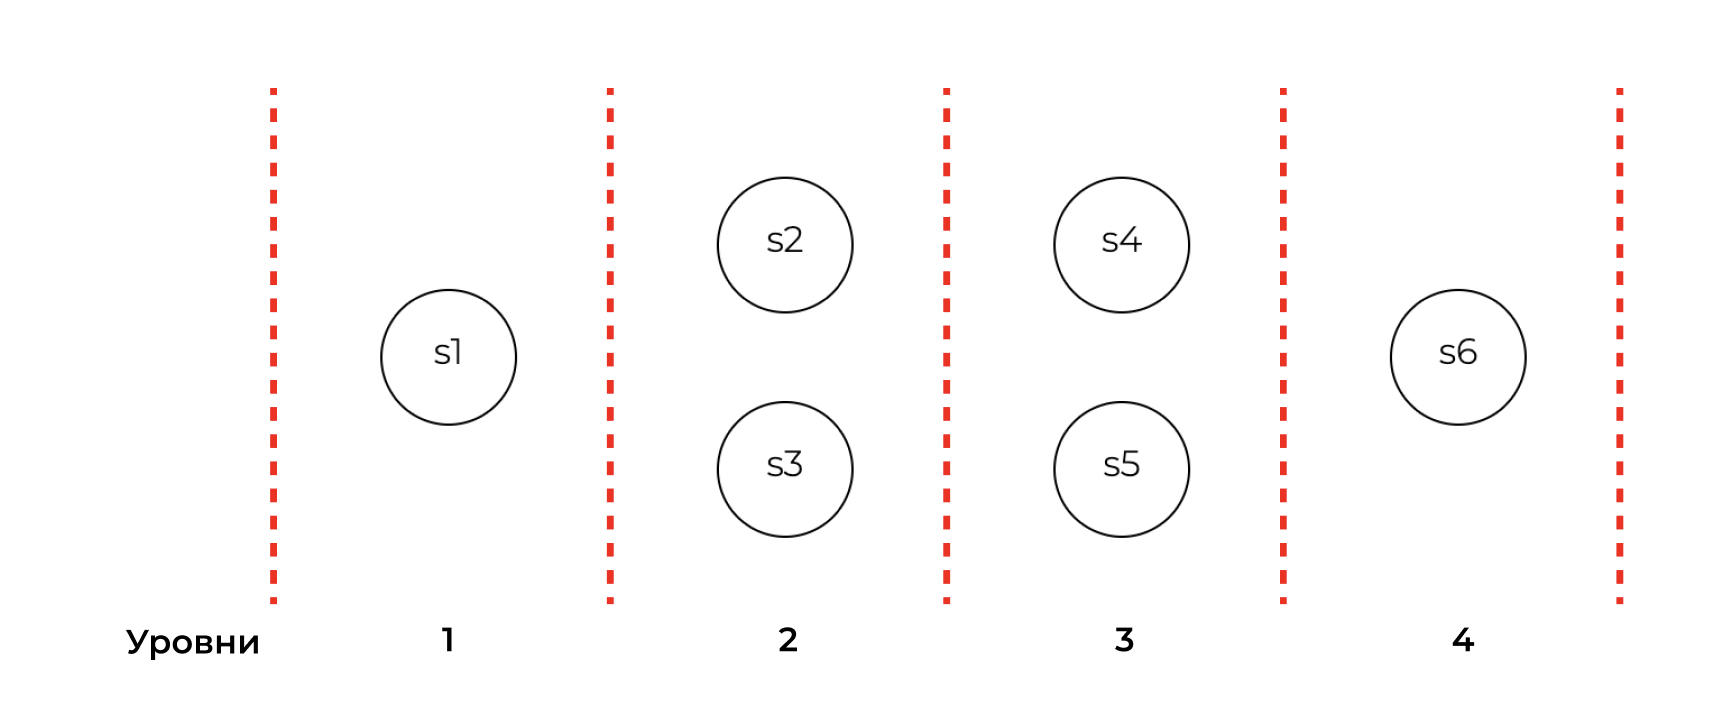
\includegraphics[width=0.9\linewidth]{images/graph_levels.png}}
\caption{Узлы графовой модели \textsf{G}, представленные на разных ``уровнях"}
\label{fig:graph_levels}
\end{figure}

~\\~\\

Разбиение графа по уровням является основой алгоритма визуализации. Рассмотрим более сложную графовую модель на языке aDOT (листинг~\ref{lst:gm.exmpl.4}).

\begin{lstlisting}[label={lst:gm.exmpl.4}, caption={Пример aDOT-определения графовой модели \textsf{TEST}}, language=JavaScript]
digraph TEST
{
// Parallelism
    s11 [parallelism=threading]
    s4 [parallelism=threading]
    s12 [parallelism=threading]
    s15 [parallelism=threading]
    s2 [parallelism=threading]
    s8 [parallelism=threading]
// Functions
    f1 [module=DEFAULT_VALUE, entry_func=DEFAULT_VALUE]
// Predicates
    p1 [module=DEFAULT_VALUE, entry_func=DEFAULT_VALUE]
// Edges
    edge_1 [predicate=p1, function=f1]
// Graph model description
    __BEGIN__ -> s1
    s6 -> s8 [morphism=edge_1]
    s7 -> s8 [morphism=edge_1]
    s10 -> s8 [morphism=edge_1]
    s11 => s8 [morphism=edge_1]
    s11 => s9 [morphism=edge_1]
    s14 -> s9 [morphism=edge_1]
    s3 -> s9 [morphism=edge_1]
    s4 => s6 [morphism=edge_1]
    s4 => s7 [morphism=edge_1]
    s4 => s10 [morphism=edge_1]
    s4 => s11 [morphism=edge_1]
    s12 => s4 [morphism=edge_1]
    s12 => s14 [morphism=edge_1]
    s13 -> s3 [morphism=edge_1]
    s15 => s14 [morphism=edge_1]
    s15 => s14 [morphism=edge_1]
    s2 => s12 [morphism=edge_1]
    s2 => s13 [morphism=edge_1]
    s2 => s15 [morphism=edge_1]
    s1 -> s2 [morphism=edge_1]
    s8 => s9 [morphism=edge_1]
    s8 => s6 [morphism=edge_1]
    s9 -> __END__ 
}
\end{lstlisting}

Полученный в результате граф представлен на рисунке (\ref{fig:main_graph}).
\begin{figure}[ht!]
\center{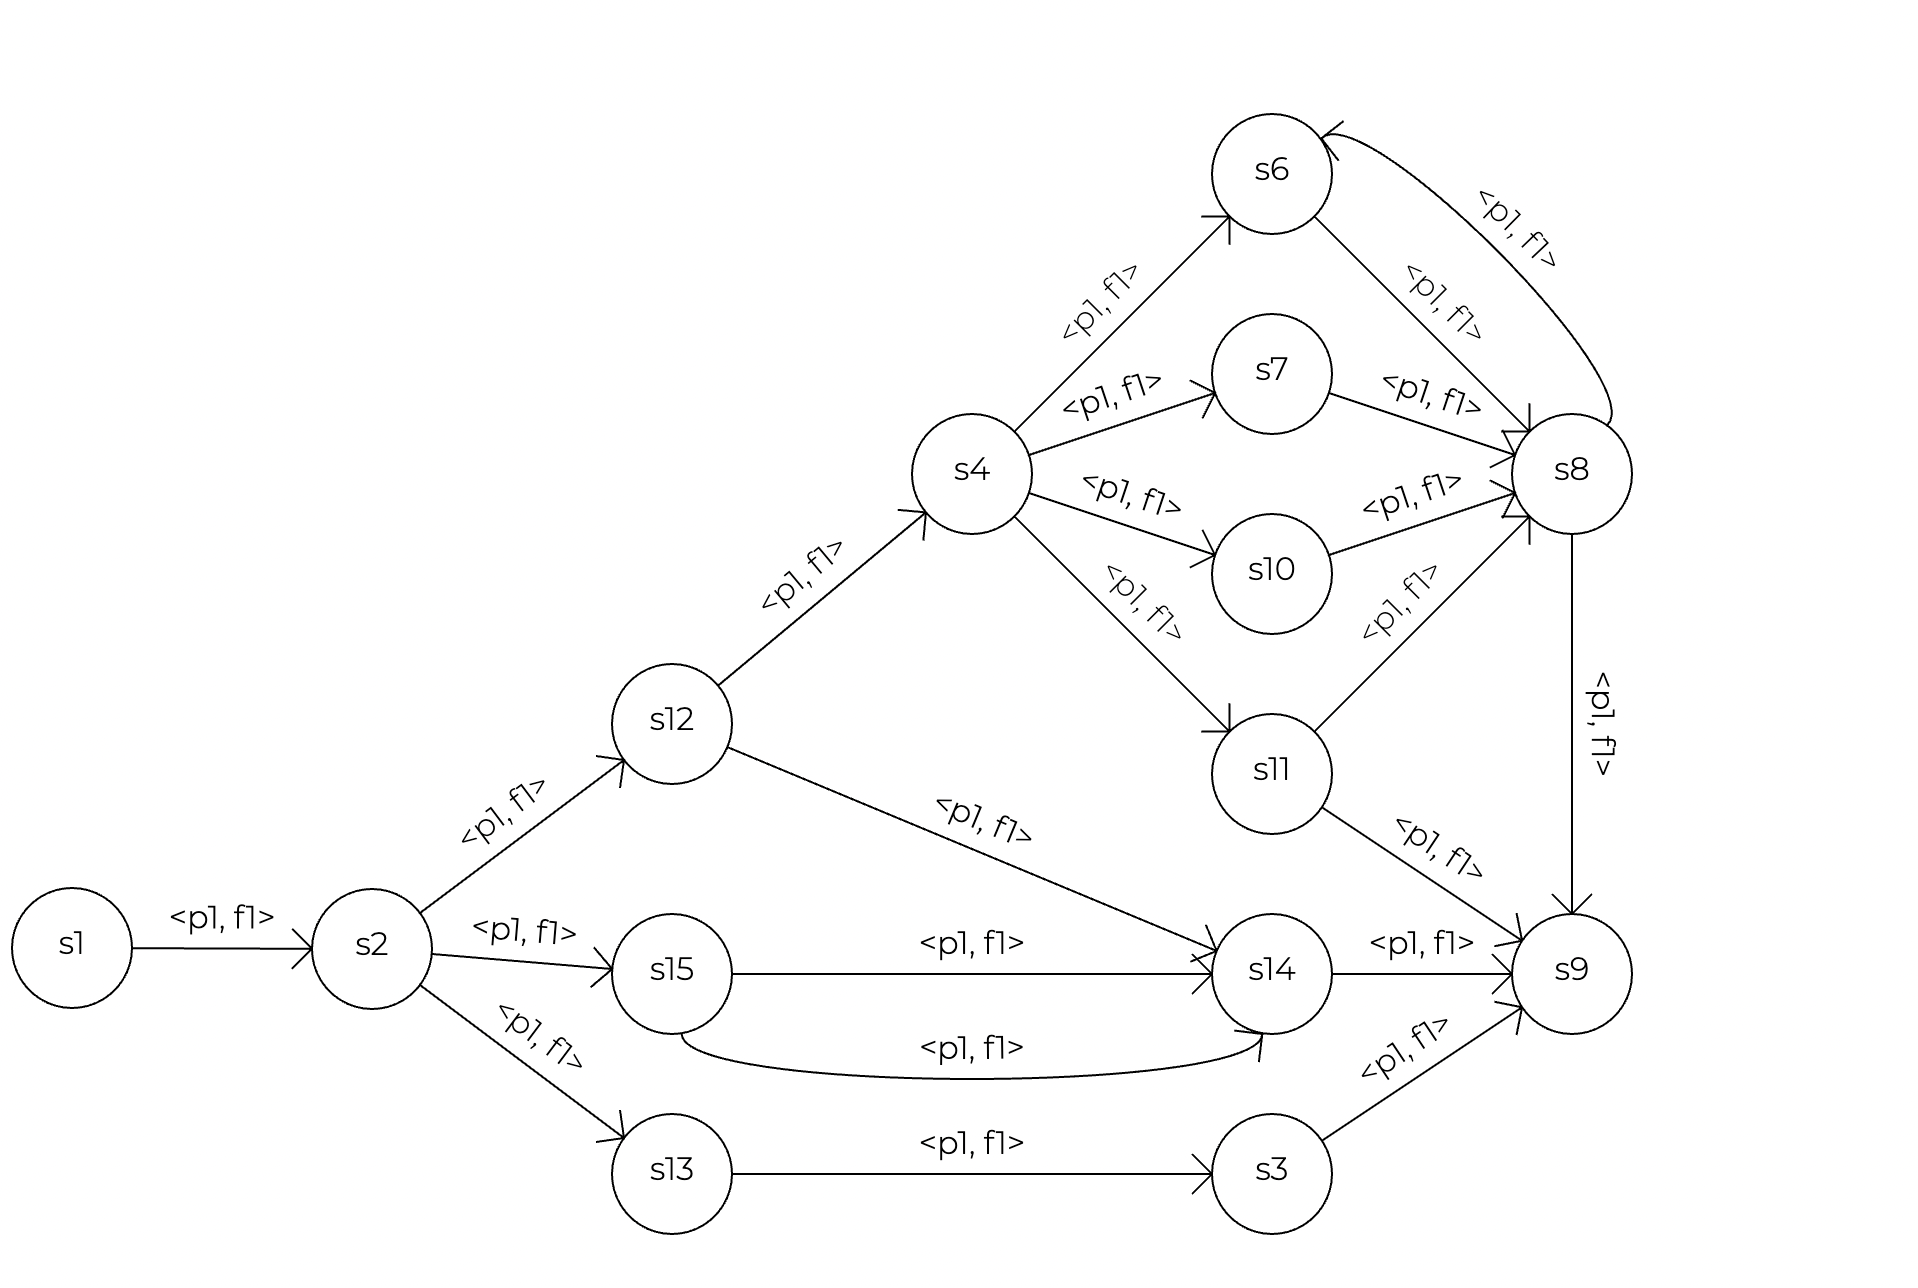
\includegraphics[width=0.9\linewidth]{images/main_graph.png}}
\caption{Визуализация графовой модели \textsf{TEST}}
\label{fig:main_graph}
\end{figure}

Алгоритм выполняется в два этапа: разбиение вершин по уровням, так, будет получено расположение вершин по координате X, затем в рамках каждого уровня распределение вершин по координате Y. Для хранения уровней вершин используется объект levels. Для рассматриваемого в примере графа после разбиения вершин объект levels содержит следующие данные (листинг~\ref{lst:gm.exmpl.5})

\begin{lstlisting}[label={lst:gm.exmpl.5}, caption={Объект levels после разбиения вершин по уровням}, language=JavaScript]
{
    "1":[{"s1":[]}],
    "2":[{"s2":["s1"]}],
    "3":[{"s12":["s2"]}, {"s13":["s2"]}, {"s15":["s2"]}],
    "4":[{"s4":["s12"]}],
    "5":[{"s9":["s14","s3"]}, {"s6":["s4"]}, {"s7":["s4"]}, {"s10":["s4"]}, 
    {"s11":["s4"]}, {"s14":["s12","s15"]}, {"s3":["s13"]}],
    "6":[{"s8":["s6","s7","s10","s11"]}, {"s9":["s11","s14","s3"]}]
}
\end{lstlisting}

Ключами объекта levels являются номера уровней, представленные в формате string. Свойствами являются массивы, на один уровень - один массив. Каждый элемент массива содержит информацию об одной вершине на этом уровне, следовательно количество вершин на уровне - это размер массива. Заметим, что элемент массива это не просто string с названием вершины, а объект. Этот объект содержит один ключ - название вершины на этом уровне, а свойством является массив, который содержит список вершин из которых перешли в эту вершину (переход только по одному ребру). В качестве примера рассмотрим уровень 5 (листинг~\ref{lst:gm.exmpl.6}) объекта levels, который был представлен ранее (листинг~\ref{lst:gm.exmpl.5}).

\begin{lstlisting}[label={lst:gm.exmpl.6}, caption={Пример уровень 5 объекта levels}, language=JavaScript]
{
    "5":[{"s9":["s14","s3"]}, {"s6":["s4"]}, {"s7":["s4"]}, 
    {"s10":["s4"]}, {"s11":["s4"]}, {"s14":["s12","s15"]}, {"s3":["s13"]}],
}
\end{lstlisting}

Уровень 5 в графе содережит следующие вершины: $s9, s6, s7, s10, s11, s14, s3$. В вершину $s6$ приходит ребро из вершины $s4$, таким образом, по ключу s6 находится массив c один элементом $s6$. На рисунке (\ref{fig:main_graph_level5}) представлен граф с выделенным уровнем 5.

\begin{figure}[ht!]
\center{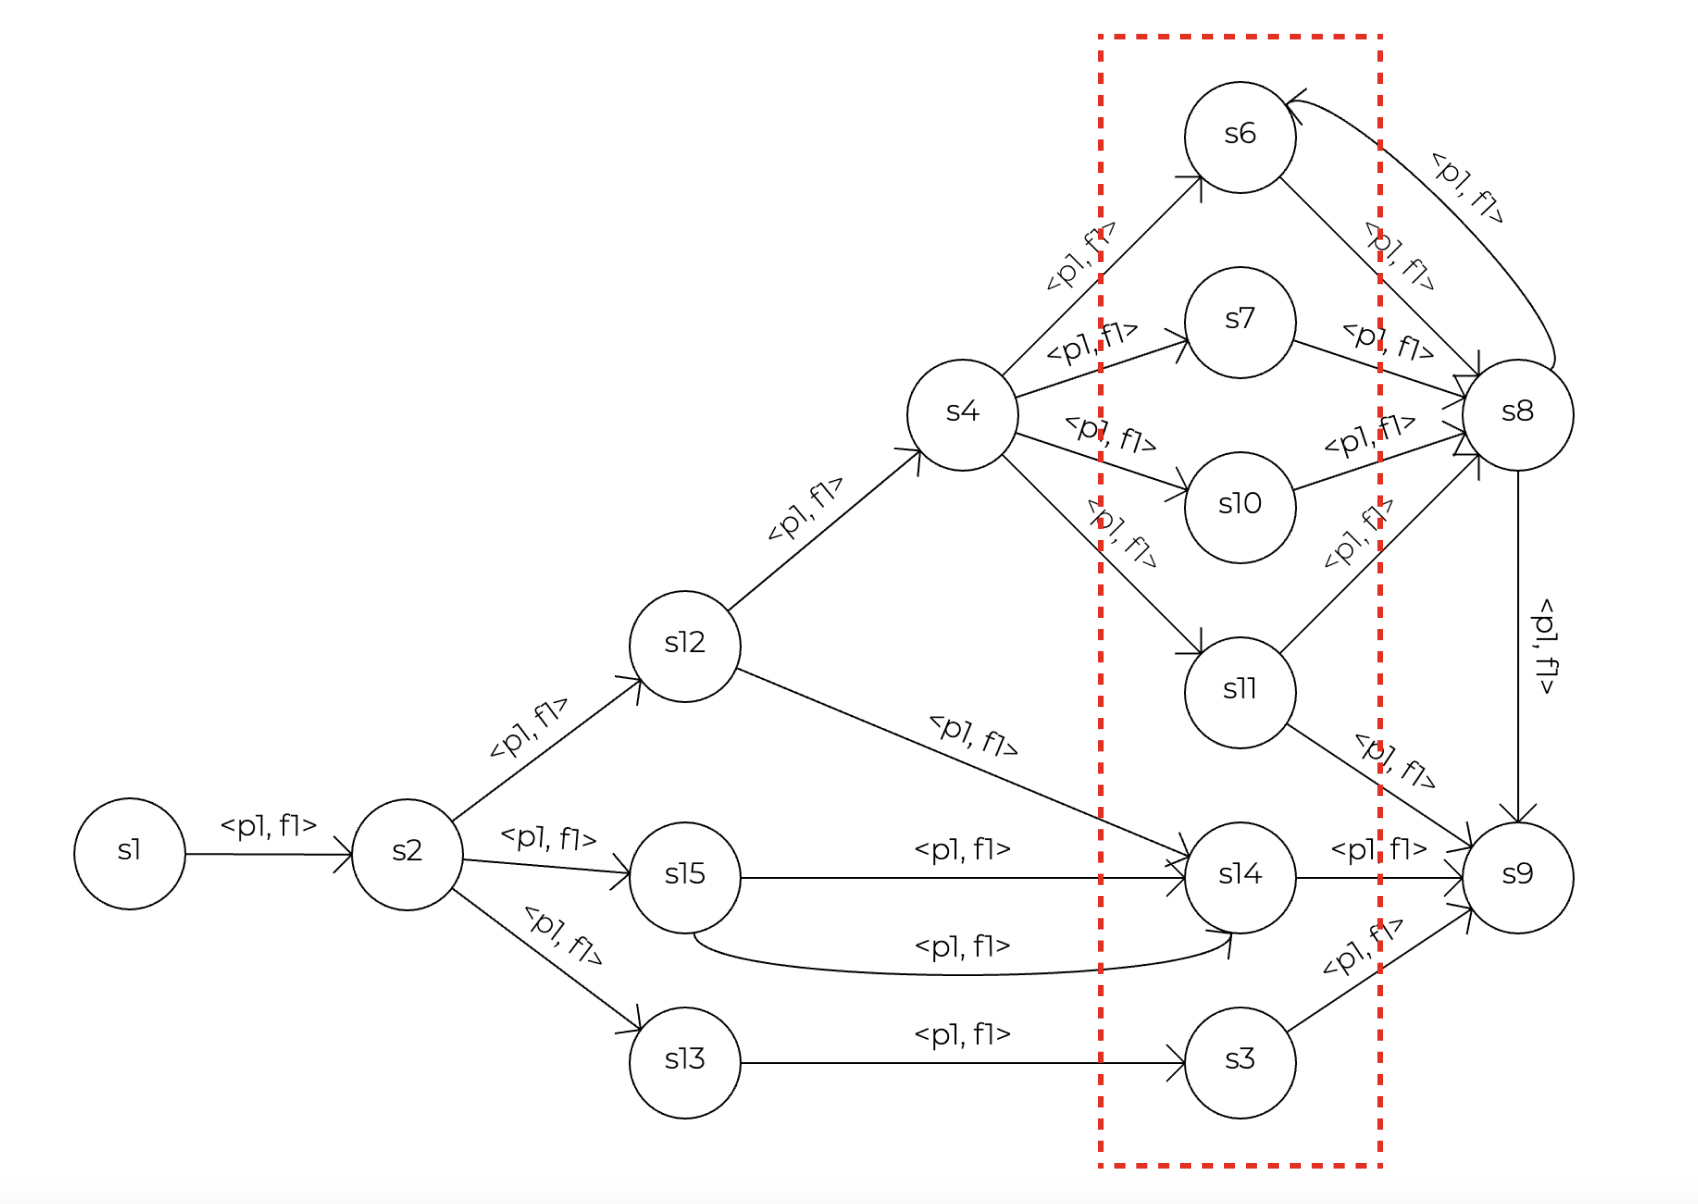
\includegraphics[width=0.9\linewidth]{images/main_graph_level5.png}}
\caption{Выделенный уровень 5 на рассматриваемом графе}
\label{fig:main_graph_level5}
\end{figure}

Обратим вниманием на то, что в объекте levels для уровня 5 содержится вершина s9 которой нет на уровне 5, а она присутствует только на уровне 6. Заполнение объекта levels происходит слево-направо, то есть от меньшего уровня к большему, например, в графе представленном выше есть связь $s13 \rightarrow s3$, таким образом пока в объект levels не будет записана вершина s13, мы не сможем записать связанную с ней вершину s3.

Обратным образом происходит дублирование вершин, если обратиться к описанию графовой модели предсталвенной выше, то можно заметить такую связь: $s1 \rightarrow s2 \rightarrow s13 \rightarrow s3 \rightarrow s9$. При начальной инициализации объекта levels $s1$ будет находиться на уровне 1, $s2$ будет находиться на уровне 2 и так далее. Таким образом, вершина $s3$ будет находиться на уровне 4 - это некорректное расположение. Для разрешения подобных коллизий после начальной инициализации объекта levels "в лоб" предусмотрено множество дополнительных проверок. Таким образом, на выходе получается корректно сформированный объект levels и сформированный объект, который будет хранить информацию о вершинах которые находятся не на своем уровне, эти вершины не будут отрисовываться, но при этом они будут учитываться при размещении по оси Y связанных с ними вершин, следовательно просто удалить такие вершины из объекта levels нельзя.

